\section{Design Overview}
\label{s:overview}

The NetMap platform is designed to be used by location-based mobile games that
measure the wireless Internet access performance as players interact with the
game's virtual world, which maps to the real world. The library's mission is to
make it as easy as possible for game developers to integrate the performance
measurement functionality in their games.

NetMap uses a dedicated server for collecting and storing the performance
measurements (see figure \ref{fig:servers}), so game developers do not need to
worry about securely storing and forwarding the sensitive data, and do not need
to provision for the bandwidth required by the data uploads.

\begin{figure}[hbtp]
  \center{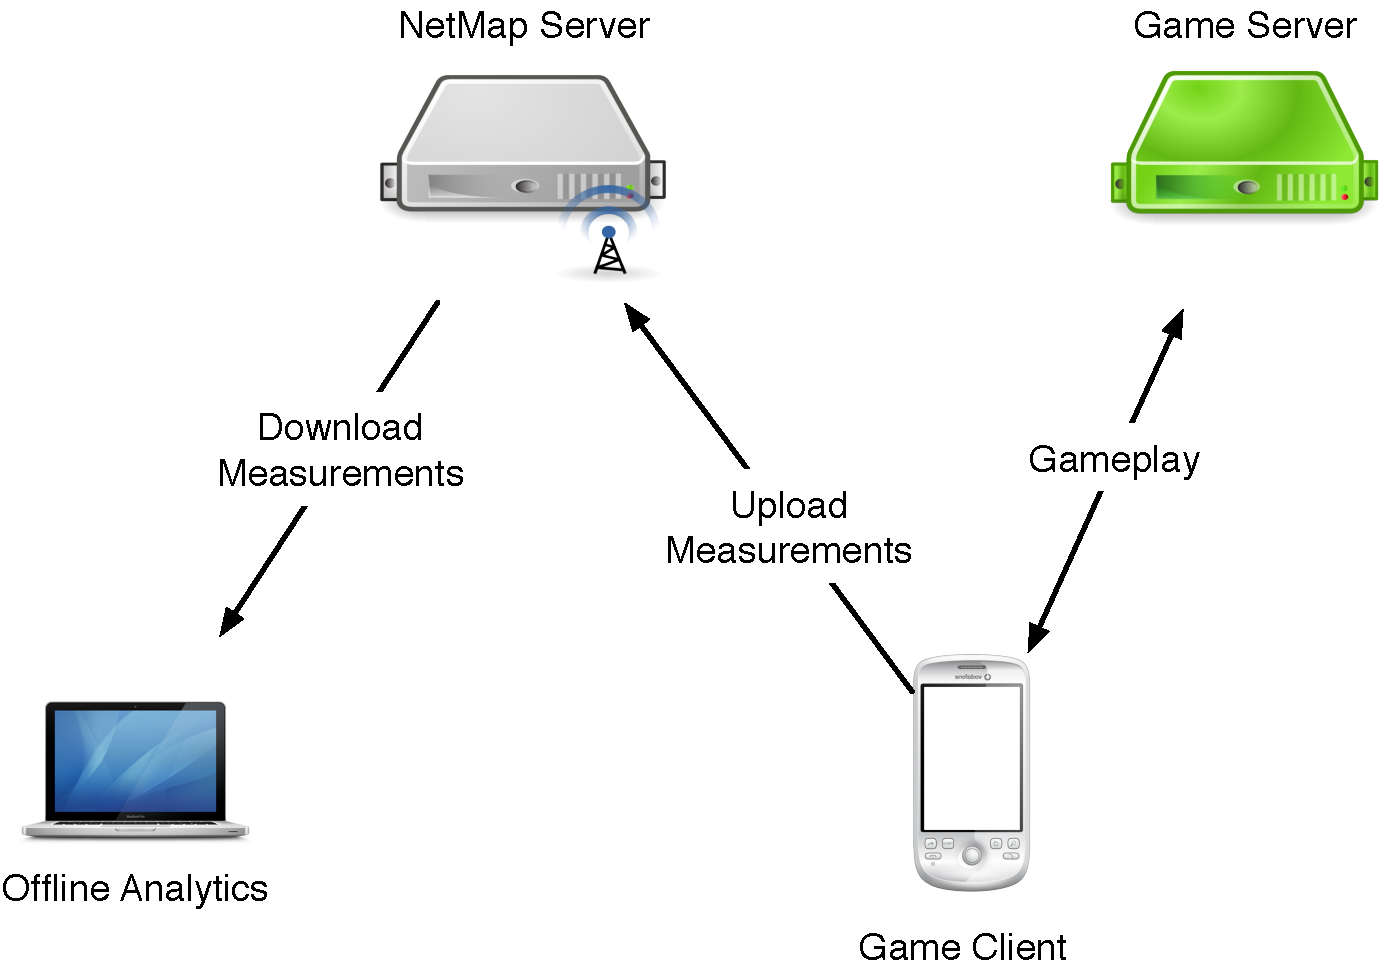
\includegraphics[width=85mm]{figures/servers.pdf}}
  \caption{
    The NetMap platform has a dedicated server for storing network
    performance measurements, and the data is analyzed offline.
  }
  \label{fig:servers}
\end{figure}

The NetMap platform includes an Android library that manages the
straight-forward (but tedious) aspects of measuring network performance and
uploading the data to the NetMap server. We envision that when a player takes
an action in a game, the game code will call our library and ask it to collect
a performance measurement. The measurement data is not uploaded to the NetMap
right away, so that the game can use all the player's (potentially limited)
wireless Internet bandwidth, so that the data upload is not charged against
the player's cellular Internet data quotas, and so that we do not burden the
player's mobile device battery. Instead, we queue up the data in a SQLite
database on the player's device, and we wait until the device is connected to a
WiFi network and its charger is plugged in. Under the right circumstances, all
the data queued up in SQLite is uploaded to the measurement server.

\begin{figure}[hbtp]
  \center{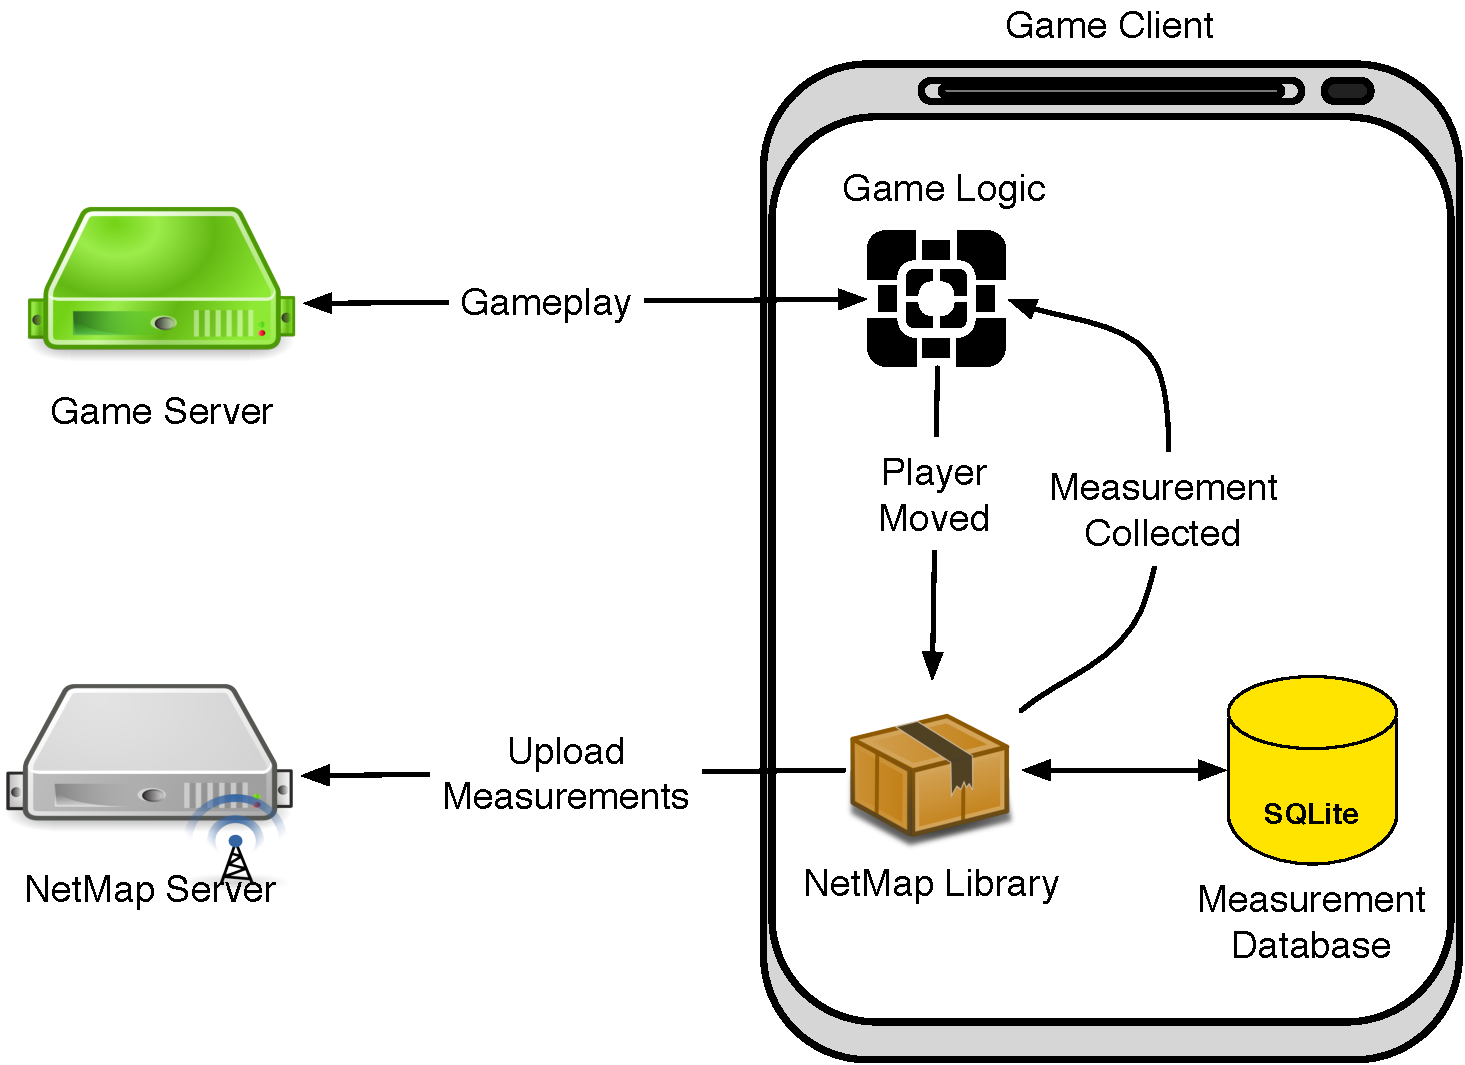
\includegraphics[width=85mm]{figures/dataflow.pdf}}
  \caption{
    The NetMap platform has a dedicated server for storing network
    performance measurements, and the data is analyzed offline.
  }
  \label{fig:dataflow}
\end{figure}


Powerful moves (such as firing a very powerful
weapon) would trigger the collection of more battery-intensive measurements.



\section{}


\subsection{Performance Measurement Data}
\label{ss:measurements}
We collect more than 200 types of network data, including device-specific data such as device model,
location data, network performance data including latency, bandwidth, and average round-trip-time,
neighboring network infrastructure information such as neighboring network type and signal strength to
neighboring towers/access points, and the DHCP information. All the data is stored in the JSON format,
because it is extensible and JSON parsers are available in many (if not all) the popular programming
languages. Section~\ref{s:appendix} presents an example of the measurement. 


{\bfseries Device-Specific Information.} \name{} collects device-specific information including the device ID
(IMEI or ESN), the device type (GSM or CDMA), the OS version. With the device ID, we can
identify a device, track the device, and discard bad data that comes due to cheating. We can
even provide personalized diaries of network usage which allow users to better understand their network
using habits.
Collecting OS version allows us to infer the effect of system and hardware on the network performance. \name{} also
logs SIM card information, such as the phone number, the SIM card operator (AT\&T, T-Mobile, etc.),
the radio type (EDGE, GPRS, HSDPA, etc.).
This permits us to create the map of network quality for each phone carrier or type, and to track how the network quality
evolves over time.

{\bfseries Location.} The system gathers the user's location information from the GPS or network location provider.
For the GPS, in addition to the latitude and longitude, our system also collects information
about the observed satellites, including the almanac, ephemeris, azimuth, elevation, and SNR.
We plan to use the satellite information to detect users that cheat the game by faking their GPS locations.
Because GPS is unavailable indoors, we also use the network location provider's estimated locations.
%gather location estimation from the network provider
%and verify its eligibility with the cell tower/AP information we collect.


{\bfseries Network Infrastructure Information.} \name{} collects information about
neighboring WiFi APs and cell towers. The cell tower information includes the mobile country code (MCC),
mobile network code (MNC), location area code (LAC), and the signal strength; the WiFi AP information
includes the MAC address, SSID, IP address, frequency band, RSSI, link speed, etc.
With the locations where users observed the cell tower/AP, we can approximate the location of
each cell tower/AP. Many research projects~\cite{ctrack, vtrack-sensys09} have focused on using
energy efficient sensors to provide accurate position estimation, but most of them suffer from
low coverage problem due to lack of cell tower/AP observations. We believe we can greatly assist those projects
with the crowd-sourced data that we have. However, neighboring GSM cell tower information isn't
universally available across all phones. Some phone models limit the cell information to only
the connected tower or do not make it available at all.

\name{} also collects the DHCP information, including the assigned IP, network mask, IP of the DHCP server, etc.
DHCP information is useful for inferring the network topology, and for cheating detection.


{\bfseries Network Performance.} We collect sophisticated network performance measurements
such as the network latency, bandwidth, average round-trip-time, and some TCP variables.
For researchers, they can use the information for research on improving network reliability and performance or
 making tradeoffs when designing systems.
For normal users, these measurements help them choose the network carrier and device which provide
 the best reception in their neighborhood.

We use the Network Diagnostic Tool (NDT)~\cite{NDT} to collect network information. NDT measures various network
performance metrics between the mobile device and their distributed servers. There are some straightforward
and incredibly tedious problems in measuring the network performance. First, in order to get individual latency
measurements for both the uplink and downlink, one needs to consider the time
synchronization problem between the device and the server. Second, to avoid variability introduced by the Internet,
one needs to maintain servers in multiple places.
NDT solves the time synchronization problem, and it maintains 81 servers in 27 countries. This allows \name{}
to provide accurate network performance measurements across the world.

\subsection{Battery/Network Awareness}
\label{ss:awareness}
There are two important aspects that designers need to take into account when implementing a mobile
programming API. First, the API should lend itself to energy-efficient applications.
Second, games using the API should avoid causing the users to incur data usage charges.

\name{} addresses these two problems by incorporating the concept of battery and network aware.
To be battery aware, \name{} monitors the battery level and status. Games using the API would get
notified when the phone is charging or when the battery level is low, and take certain actions
to save energy. For example, if the phone is charging, the game can start uploading the measurements
it collected to the server or taking measurements more frequently.

\name{} is also network aware. \name{} monitors the network type that the device is currently using,
and notifies the games that using the API if the user switches to either WiFi or cellular network.
Games can react to the notification by uploading all the collected measurements to the server when
the phone is using WiFi.


\subsection{Algorithm}
\label{ss:algorithm}
From the large amount of data we collect, we can infer several characteristics of
wireless networks and their infrastructures. One such characteristic is the location
of cell towers that users either connect to or are in the vicinity of, since we collect
neighboring cell tower information. We tried two different algorithms for cell tower
positioning which are described below. Each algorithm uses multiple readings to
position a given cell tower. For each algorithm, we use the following abbreviations:
Location of reading = L^MLocation of cell tower = T^MDistance = L - T = d^MSignal strength = s
^M
{\bfseries Algorithm 1- Channel Model Estimation}
We begin with the common model for wireless network channels: s \propto \frac{k}{d^2}
where k is the channel condition parameter. However, we donÕt know the channel
condition parameter and it is difficult to accurately estimate. We do know that readings
in similar locations should have similar channel condition parameters so we disregard
k (since it is roughly constant across readings in same location at similar time) and state:

s \propto \frac{k}{d^2} \rightarrow d^2 = \frac{1}{s} \rightarrow d = \sqrt{\frac{1}{s}} \rightarrow L - T = \sqrt{\frac{1}{s}} \rightarrow T = L - \sqrt{\frac{1}{s}}

To obtain cell tower location, we solve for T in each reading and use the location which solves
min(sd^2 Ð 1), which is derived from minimizing d^2 = \frac{1}{s} (so sd^2 Ð 1 \approx 0)


{\bfseries Algorithm 2- Weighted Average of User Locations}
We assume that users that connect or detect a cell tower with reasonable signal strength
are relatively close to the tower. Since all user locations, after eliminating outliers, will be
a small distance from the cell tower, and each will have a different orientation with respect
to the cell tower, we weight each reading by signal strength and sum the locations to obtain
an estimate of the cell tower location.

We first, for all entries, eliminate those with signal strength below a threshold. This eliminates
the use of outliers since very low signal strength implies that the user is not very close to the
cell tower being considered. We then weight each readingÕs location (longitude and latitude separately) by:
\frac{signal strength of current reading}{sum of signal strengths from all readings above threshold}
Finally, we add the weighted longitudes and the weighted latitudes to obtain an estimate on the location
of the cell tower. The accuracy of this algorithm grows as more readings are used.



